\chapter{Methodology}

Students participated in five 90-minute activity sessions, once per week, for five consecutive weeks. Each session presented one activity that was intended to exercise different engineering and design principles. Students were observed and video recorded as they carried out the activities. 

\section{Subject Selection} 

This study used seven middle-school students as subjects. Students were in grades seven and eight, with average age of approximately 12 years old. The students reported that the grades they received in school were average or better, with the centroid of the distribution being `B' marks. The selection process was done by an after school enrichment program, where this study was advertised as an activity in which students could elect to participate.  This enrichment program served students from a region that is academically under-performing.  The students were nominated by a teacher or administrator for having talent for learning, even if the students' grades do not reflect that talent. Five of the six students identified themselves as a minority race. This study was open to all students of the specified grade levels who were active in the after school program. Selection was simply the first students to volunteer to participate.

All students read, understood, and signed a student assent form and their guardians read, understood, and signed a parental consent form (see Appendix~\ref{sec:parent_consent}). Parental consent forms were available in English and Spanish. The student assent form was available only in English, as that is the language the research activities were conducted in. Guardians had the option to sign a media release form, which allowed recorded media of their child to be used in publication. 

\section{Session Protocol}

In each session, students engaged in an engineering and design activity. Their conversations, problem-solving strategies, and concluding interviews were observed in person by researchers and video recorded for later analysis.

Each of the five sessions followed the same agenda. Students arrived and were brought to a conference room for snack time, where they were casually introduced to the concepts involved in that day's activity. Loud thinking protocol, in the style of TAPPS, was explained and reinforced every week at this time. Loud thinking is a process of talking through one's thoughts as a stream of consciousness \citep{lochhead87}. After about twenty minutes in the conference room, the students moved to the activity room where the apparatus for that day's study was set up. Working in pairs, students worked through the prescribed activity. The entire time in the activity room was  audio and video recorded. Throughout the activity students were prompted by researchers to explain their thoughts, ideas, and understanding of concepts.

At the conclusion of the activity, students were led in a group conversation about what they learned and developed. These conversations were also recorded. The questions asked by researchers during this conversation were variations of:
\begin{itemize}
\item What did you do to find your solution?
\item Did you do anything early on that you did again to help yourself?
\item If you had a friend who was coming in to work on this problem tomorrow,
what would you recommend they do?
\item Are there any other tricks you discovered?
\end{itemize}

%%%%%%%%%%%%%%%%%%%%%%%%%%%%%%%%%%%%%%%%%%%
%%%%%%%%%%%%%%%%%%%%%%%%%%%%%%%%%%%%%%%%%%%
\section{Design of Activities}
\begin{table}
\begin{centering}
	\begin{tabular}{c  c   c}
	Week & Activity & Related Field \\ \hline
	1 & ``Rush Hour" Game & math problem solving \\ 
	2 & Light Optimization & electrical engineering \\ 
	3 & Gear Reduction & mechanical engineering \\ 
	4 & Word Search & computer science \\ 
	5 & Elevator Control & computer science \\ \hline
	\end{tabular}
	\caption[List of design activities.]{List of design activities, in order that they were conducted by students, with their related field.}
	\label{tab:activity-list}
\end{centering}
\end{table}

The activities performed by the students were designed in advance to cover a large sample of design problems.  Each activity stressed different areas of engineering space, starting with a simple activity and progressing towards complex algorithm design. In total, the activities are intended to support computational thinking, as discussed in Chapter~\ref{chap:background}.  The activities were performed a week apart from each other, which allowed for changes to be made to the activity plans based on preceding sessions. Every activity represented a real engineering or design problem, had observable iteration behavior, defined metrics of success, and were process-oriented, as discussed in Section~\ref{sec:MEA}.

Subject areas of activities included:
\begin{description}
\item [Parallel and series circuits:] the two fundamental arrangements of resistive components in electrical circuit design, their properties, and their tradeoffs. 
\item [Gear ratios and reduction:] the combination of different sized gears to convert between high-speed and high-torque, used in most motor applications.
\item [Algorithm design:] the design of a processes or set of rules that can be executed on a data set to arrive at a particular solution.
\item [String-matching:] a category of problems that involve identifying sequences of characters within a greater set. 
\item [Active control systems:] a category of systems that use real-time feedback, typically to control a moving machine.
\end{description}
In addition to subject areas, the activities stressed different elements of design skills:
\begin{description}
\item [Balancing between contradicting requirements:] a common problem in engineering, where satisfying two requirements simultaneously is impossible, and a compromise must be considered.
\item [Working within time constraints:] the skill of assessing how deeply a problem can be examined in the amount of time provided as not to be unfinished at the conclusion of that time.
\item [Physical construction:] a difficult task in general.
\item [Symbolic manipulation of a system:] performing design tasks abstractly by use of generalized symbols.
\end{description}


 
 \label{sec:success-levels}
Each activity had two levels of success. The first level is the completion of a successful design that solves the problem. The second level is synthesizing a general process for arriving at a solution. Both levels are defined as success criteria for each activity in the following sections. The five activities are now presented. They are also summarized in Table~\ref{tab:activity-list}.

%%%%%%%%%%%%%%%%%%%%%%%%%%%%%%%%%%%%%%%%%%%Rush Hour
\subsection{Week 1: Rush Hour}
	
	``Rush Hour" is a sliding tile game where the player must manipulate cars on a small grid. The object of the game is to slide the cars so that the target car, indicated in Figure~\ref{fig:rushhourgame} by the arrow,  can escape through the opening at the right side of the game board.  The game has a small set of simple rules, but a high number of possible states for any given puzzle. Every time a piece is moved, the game is considered to be in a different state. Certain states are only accessible from other specific states. For example, the top-left car in Figure~\ref{fig:rushhourgame} can only be moved to the top-right position after the truck in the upper-right has been moved out of the way. All of the states in which that car is in the top-right position are only accessible through a selection of states where the truck has been moved. The total number of states possible for this game is the total number of unique combinations that the cars can be arranged in, which is large space.
	
		\begin{table}
	\begin{centering}
	\begin{tabular}{l  l   l}
		\multicolumn{3}{l}{{\large Rush Hour Specifications}} \\
		\toprule
		\multirow{2}{*}{Success Criteria}  
			& Solution: 		& Solved puzzle \\ \cmidrule(r){2-3}
			& Process:		& Described Strategies \\ \midrule
		Iteration Metric	 & \multicolumn{2}{c}{Backtracking or resetting: deviation from current course }\\ 
		\bottomrule
	\end{tabular}
	\caption{Rush Hour activity success and iteration criteria.}
	\label{tab:spec-rush-hour}
	\end{centering}
	\end{table}
	
	\subsubsection{Purpose}
	
	This activity was an ideal introductory experience for the students. It had few rules to learn and was fun to play. Students were quickly engaged; most of them had played the game before. As a design activity, this provided observations of the students' methods in navigating large number of possible states of the game. With every move of a game piece, the possible states accessible on the next move change. Many times, the path the player is on does not have a solution, and the player must backtrack to reach an earlier state where a different decision could yield a solution, or, start over and try again. This property is known as a ``deep state space." The backtracking behavior was a primary component of the analysis of this activity.
	
	Welch cited \citet{ericsson-1984} with the importance of a warm up process, stating that when verbal information exchange is involved, a period of warm-up is necessary for the subject and researcher to communicate most effectively. This activity, with its simple rules and familiarity, provided an opportunity for students to focus on the loud thinking strategy, warming up that skill for the remaining sessions.
	
	\subsubsection{Protocol}
	
	%
	\begin{figure}
	\begin{centering}
	\includegraphics[height=0.35\textheight]{images/rushour-2}
	\par\end{centering}
	\caption[Rush Hour game board.]{Rush Hour game board. The arrow indicates the target car.}
	\label{fig:rushhourgame}
	\end{figure}
	
	The students were each given a game unit with a beginner-level puzzle to solve.  The students were encouraged to {}``think out loud'' during the entire process, and to think about the process they were employing to arrive at solutions.
	
	Once the students felt that they understand the concept of the game, they were put into pairs and given a more difficult puzzle. During this phase, a camera was positioned above the table to record the game board, the students' hands,
	and the students' voices. Additional puzzles of increasing difficulty were used as time allowed.
	
	During the session students were asked to identify the ``key move" of puzzles that they had solved. The ``key" is the critical move that unlocks the puzzle, allowing it to be solved very easily.
	
	At the conclusion of the puzzle solving session, the student pairs were asked to explain the process of solving the puzzle. The students were instructed to explain their process of finding a solution, not the steps to carry out a specific solution. They were then instructed to explain the game strategy for a friend who had not seen the game previously.
	
	A semi-structured interview was used to probe students\textquoteright{} understanding. The interview was based on these questions:
	\begin{itemize}
	\item Please explain what you did to find the solution to these puzzles. 
	\item Did you do anything in the first puzzle that you did again in the
	second to help yourself out? 
	\item I want you to explain how to go about solving these kinds of puzzles.
	Pretend you\textquoteright{}re explaining it to a friend who has never
	done this before. 
	\item Are there any tricks you discovered? 
	\end{itemize}
	
	\subsubsection{Rationale}
	
	The Rush Hour game was characterized by its large state space, as discussed above. Trying to solve it led to a rapid iteration of ideas and high degree of backtracking. This type of problem is common in computer science and mathematics, and can be generalized to include other games (such as chess) as well as real engineering problems. For example, circuit board routing is a design activity that has a large number of states where decisions progressively lead to new areas of the state map, fitting this general problem type.

\begin{table}
	\begin{centering}
	\begin{tabular}{l  l   l}
		\multicolumn{3}{l}{{\large Light Optimization Specifications}} \\
		\toprule
		\multirow{2}{*}{Success Criteria}  
			& Solution: 		& Built working circuit (plus formulaic score) \\ \cmidrule(r){2-3}
			& Process:		& Reasoning for design \\ \midrule
		Iteration Metric	 & \multicolumn{2}{c}{Turning on power supply }\\ 
		\bottomrule
	\end{tabular}
	\caption[Light Optimization activity success and iteration criteria.]{Light Optimization activity success and iteration criteria. The solution criteria of building a working circuit is evaluated as true or false, but this activity is unique among those in this study in there is additionally a numerical score associated with the solution.}
	\label{tab:spec-lights}
	\end{centering}
	\end{table}
%%%%%%%%%%%%%%%%%%%%%%%%%%%%%%%%%%%%%%%%%%%Lights
\subsection{Week 2: Light Optimization}
	
	The Light Optimization problem explored basic electrical principles and required students to balance between contradicting requirements. Students were presented with eight small light bulbs and a power supply. The design task was to connect the lights with alligator clip wires in a way that minimized cost without sacrificing brightness. 
	
	In the problem specification, wires and volts had costs associated with them.  The students were given a scenario that they work for a power company, and each light bulb represents a house that they service. They needed to
	find a method to light all of the homes at the lowest cost to the company. Example student work is shown in Figure~\ref{fig:lightsdesk}.

	
	\subsubsection{Purpose}
	
	\begin{figure}
	\begin{centering}
	\includegraphics[width=\textwidth]{images/lights-desk}
	\par\end{centering}
	\caption[Example of a solution to the Light Optimization activity.]{Example of solution to the Light Optimization activity. The lights are strung together in series by alligator clips.}
	\label{fig:lightsdesk}
	\end{figure}
	
	This activity generated observations of students exploring natural phenomena and balancing requirements for an optimal solution. A formula generated a cost per solution score, but students were allowed to construct arguments for the optimality of their solution. This
	was intended to further promote loud thinking and give insight to the student's thought processes.
	
	\subsubsection{Protocol}
	
	During the initial snack time, a researcher led a conversation about what ``optimization'' means, soliciting suggestions from the students. Once in the classroom, the students were presented with a workstation for each dyad. Each workstation had a variable DC power supply, a number of small, low-power light bulbs (holiday mini-bulbs), and connecting wires with alligator clips. Two workstations were initially set up with example circuits. One example was four lights connected in series, such that the same current flowed through all the lights, with the power supply operating at 12 volts. The other station had the same number of lights connected in a parallel configuration, such that every light had full voltage from the power supply, which operated at 3 volts. The two systems were approximately the same brightness. The terms {}``series'' and {}``parallel'' were never used with the students.
	
	The students were presented with a set of criteria for assessing their solutions. The goal was stated to achieve ``reasonable brightness.'' Costs were associated for number of wires used and amount of voltage required. The final cost of a solution was \[
	\frac{a \cdot \text{wires} + b \cdot \text{voltage}}{\text{number of lights}}\]
	where $a$ is the cost of wires and $b$ is the cost per volt. The students were provided with this formula at the beginning of the session.
	
	The students, working in pairs, solved two iterations of this
	activity. The two iterations had different material costs. The
	change in cost values was designed to obsolete the first iteration's
	optimal solution, forcing reconsideration of the problem.
	
	At the conclusion of the second problem iteration, the students, in
	pairs, were asked to document their solutions and explain how they
	arrived at them. They were instructed to explain their process
	as if for a friend who was not present. Interview questions examined
	the students grasp of the electrical principles, what they considered
	to be {}``optimal,'' and how they went about discovering what they
	needed to know in order to solve the problem.
	
	
	\subsubsection{Rationale}
	
	The electrical concepts in this activity were fundamental to an understanding
	of electricity and electronics, which creates the physical basis of computing
	technology. The problem was also multi-dimensional, with number of
	connections, voltage, and number of lights serving as related but confounded design parameters \citep{axiomatic}. This activity emulates real-world design problems that require simplification,
	satisficing, or constraint of solution space.

%%%%%%%%%%%%%%%%%%%%%%%%%%%%%%%%%%%%%%%%%%%Gears
\subsection{Week 3: Gear Reduction}

	In this activity the students built a transmission from LEGO
	Technic gears and components between a fixed motor and load. 
	
	\begin{table}
	\begin{centering}
	\begin{tabular}{l  l   l}
		\multicolumn{3}{l}{{\large Gear Reduction Specifications}} \\
		\toprule
		\multirow{2}{*}{Success Criteria}  
			& Solution: 		& Built transmission that lifts mass \\ \cmidrule(r){2-3}
			& Process:		& Non-trivial suggestions for a friend \\ \midrule
		Iteration Metric	 & \multicolumn{2}{c}{Applying energy to system, either by hand or by motor}\\ 
		\bottomrule
	\end{tabular}
	\caption{Gear Reduction activity success and iteration criteria.}
	\label{tab:spec-gears}
	\end{centering}
	\end{table}
	
	\subsubsection{Purpose}
	
	This problem allowed for direct access to the students' spatial and
	mechanical reasoning skills, a domain used heavily in many different
	areas of design.
	
	
	\subsubsection{Protocol}
	
	The students were introduced to the concepts of gear reduction,
	specifically the nature of ``little-to-big'' relationships \citep{ArtofLEGO}.
	Each student dyad was supplied with a workstation apparatus, constructed
	of LEGO Technic with a motor, a support structure on which to build their
	transmission, and an output pulley. The pulley was connected to
	an interchangeable mass. The students were presented with two different
	tasks, and asked attempt either one or both:
	\begin{enumerate}
	\item Lift the greatest amount of weight possible.
	\item Lift a specific weight from the floor as quickly as possible.
	\end{enumerate}
	The students had all the remaining time to design and build
	their solutions. Paper was provided, and students were encouraged
	to document their transmissions in the same fashion as was used in
	the concept tutorial.
	
	At the conclusion of the work time, each dyad's construction was tested individually as the group observed.
	
	
	\subsubsection{Rationale}
	
	This activity was an engineering design task. The requirements were simple,
	and the constraints needed to be discovered by the students. This activity was more than just a gear design test; it required construction of a stable structure which is alone a significant task. The solution was open-ended, as the gears and other components could be assembled in nearly infinite configurations, many of which may solve the problem. This activity stressed implementation and time management. 

%%%%%%%%%%%%%%%%%%%%%%%%%%%%%%%%%%%%%%%%%%%Word Search
\subsection{Week 4: Word Search}

	\begin{table}
	\begin{centering}
	\begin{tabular}{l  l   l}
		\multicolumn{3}{l}{{\large Word Search Specifications}} \\
		\toprule
		\multirow{2}{*}{Success Criteria}  
			& Solution: 		& Created steps to solve puzzle \\ \cmidrule(r){2-3}
			& Process:		& Same as Solution \\ \midrule
		Iteration Metric	 & \multicolumn{2}{c}{Testing modification to algorithm }\\ 
		\bottomrule
	\end{tabular}
	\caption[Word Search activity success and iteration criteria.]{Word Search activity success and iteration criteria. This activity is unique in that the solution and process are the same: the student's desired product is not a solved puzzle but the algorithm to solve the puzzle.}
	\label{tab:spec-word-search}
	\end{centering}
	\end{table}
	
	Students designed algorithms to solve word searches, where words
	were hidden in a two-dimensional grid of otherwise random letters.
	This activity introduced the concept of algorithm design. The puzzle and worksheets can be seen in Appendix~\ref{sec:wordsearchhandout}.
	
	\subsubsection{Purpose}
	
	The concept of an algorithm was introduced in this activity, which
	was also used in the following activity. As such, this activity partially functioned as a warm up to the more complex elevator
	control algorithm activity. 
	
	This activity allowed observations of students process in deducing
	and applying patterns, and observed students' approaches to writing
	generalized procedures.
	
	
	\subsubsection{Protocol}
	
	This protocol was implemented as a worksheet for students, as can
	be seen in Appendix~\ref{sec:wordsearchhandout}. The concept of an
	algorithm was introduced with the game of tic-tac-toe as example.
	The students were given the instruction set to never lose tic-tac-toe,
	and were encouraged to study and try it. Once the concept of using
	instructions to play a game had been mastered, the students were
	given a very simple word search puzzle. The example puzzle was
	designed to be nearly trivial, and is shown in Figure~\ref{fig:Example-word-search}.
	The words hidden in this puzzle are \emph{ace}, \emph{fire}, \emph{shoe},
	\emph{tour}, and \emph{yes}.
	
	
	\begin{figure}
	\begin{centering}
	\begin{tabular}{|c|c|c|c|c|}
	\hline 
	Y & E & S & L & F\tabularnewline
	\hline
	\hline 
	M & N & H & R & I\tabularnewline
	\hline
	\hline 
	P & T & O & U & R\tabularnewline
	\hline
	\hline 
	A & C & E & M & E\tabularnewline
	\hline
	\end{tabular}
	\par\end{centering}
	
	\caption{Example word search puzzle provided to students.}
	\label{fig:Example-word-search}
	\end{figure}
	
	The students were prompted at this point with questions, which
	were discussed briefly as a group. The questions were:
	\begin{itemize}
	\item Did you find all the words?
	\item What did you do to find the words?
	\item Did the words just ``jump out at you?'' 
	
	\begin{itemize}
	\item What if they didn't?
	\item How can you know for sure you found \emph{all} the words?
	\end{itemize}
	\end{itemize}
	The students were then prompted to write down any rules or strategies
	they employed in the example puzzle. 
	
	The researcher explained that computers are devoid of the pattern
	recognition ability that makes words {}``jump out'' for people.
	However, computers are very fast at simple computation, so they are
	advantageous to use for extremely large data sets. This provided
	impetus for the students to develop an algorithm rather than simply
	solving the puzzle one time.
	
	The students were then given the difficult puzzle, which can be
	seen in Appendix~\ref{sec:wordsearchpuzzle}. The students were encouraged
	to continue talking through their thought process, and reminded that
	the process to solve the problem was desired, not the solution itself.
	If the students completed the puzzle and were confident in the rules
	they had written, they were given an additional puzzle with the
	instructions to solve it only by following their rules, not using
	their human abilities.
	
	
	\subsubsection{Rationale}
	
	This activity stressed computational thinking, which caused students to think algorithmically about a normally straightforward task. This activity also had opportunity for cleverness and creativity that arose from noticing patterns in data. These skills are fundamental to computer science. 

%%%%%%%%%%%%%%%%%%%%%%%%%%%%%%%%%%%%%%%%%%%Elevator
\subsection{Week 5: Elevator Control}

	\begin{table}
	\begin{centering}
	\begin{tabular}{l  l   l}
		\multicolumn{3}{l}{{\large Elevator Control Specifications}} \\
		\toprule
		\multirow{2}{*}{Success Criteria}  
			& Solution: 		& Wrote control program that operates successfully \\ \cmidrule(r){2-3}
			& Process:		& Useful recommendations for a friend \\ \midrule
		Iteration Metric	 & \multicolumn{2}{c}{Running program }\\ 
		\bottomrule
	\end{tabular}
	\caption{Elevator Control activity success and iteration criteria.}
	\label{tab:spec-elevator}
	\end{centering}
	\end{table}
	
	Elevators are robotic devices that need to act based on multiple inputs and system states, and require well-thought-out control algorithms to function effectively. In this activity, students designed a set of rules to govern the motion of a simulated elevator. The simulation acted as a microworld, allowing students to experiment with a controlled subset of problem physics \citep{levin87}. The simulated elevator was implemented in Scratch using the BYOB extension, allowing for custom drag-and-drop code blocks for high-order control of the graphical elevator system \citep{scratch, byob}.
	
	The workspace for the microworld is shown in Figure~\ref{fig:elevator-workspace}. The representation of the building is the white panel on the right. The red rectangle (d) is the elevator car, shown at rest on the first floor. The floors are delineated by light-colored lines, and each has a gray, circular call button (e). At the far right of the white panel is a gray inset panel that contains a queue of floor requests as the simulator runs (f). The simulator automatically places a request on the queue when a floor button is clicked by the user. 
	
	Code is written by dragging primitives and control structures from the left panel to the center panel. In the center panel, the primitives can be assembled to form command, query, and repetition sequences. A set of procedures were made for the purpose of elevator control and were added to the palette. The custom procedures are shown in in Figure~\ref{fig:elevator-blocks}.
	
	\begin{figure}
	\begin{centering}
	%\includegraphics[width=\textwidth]{images/elevator-workspace}
	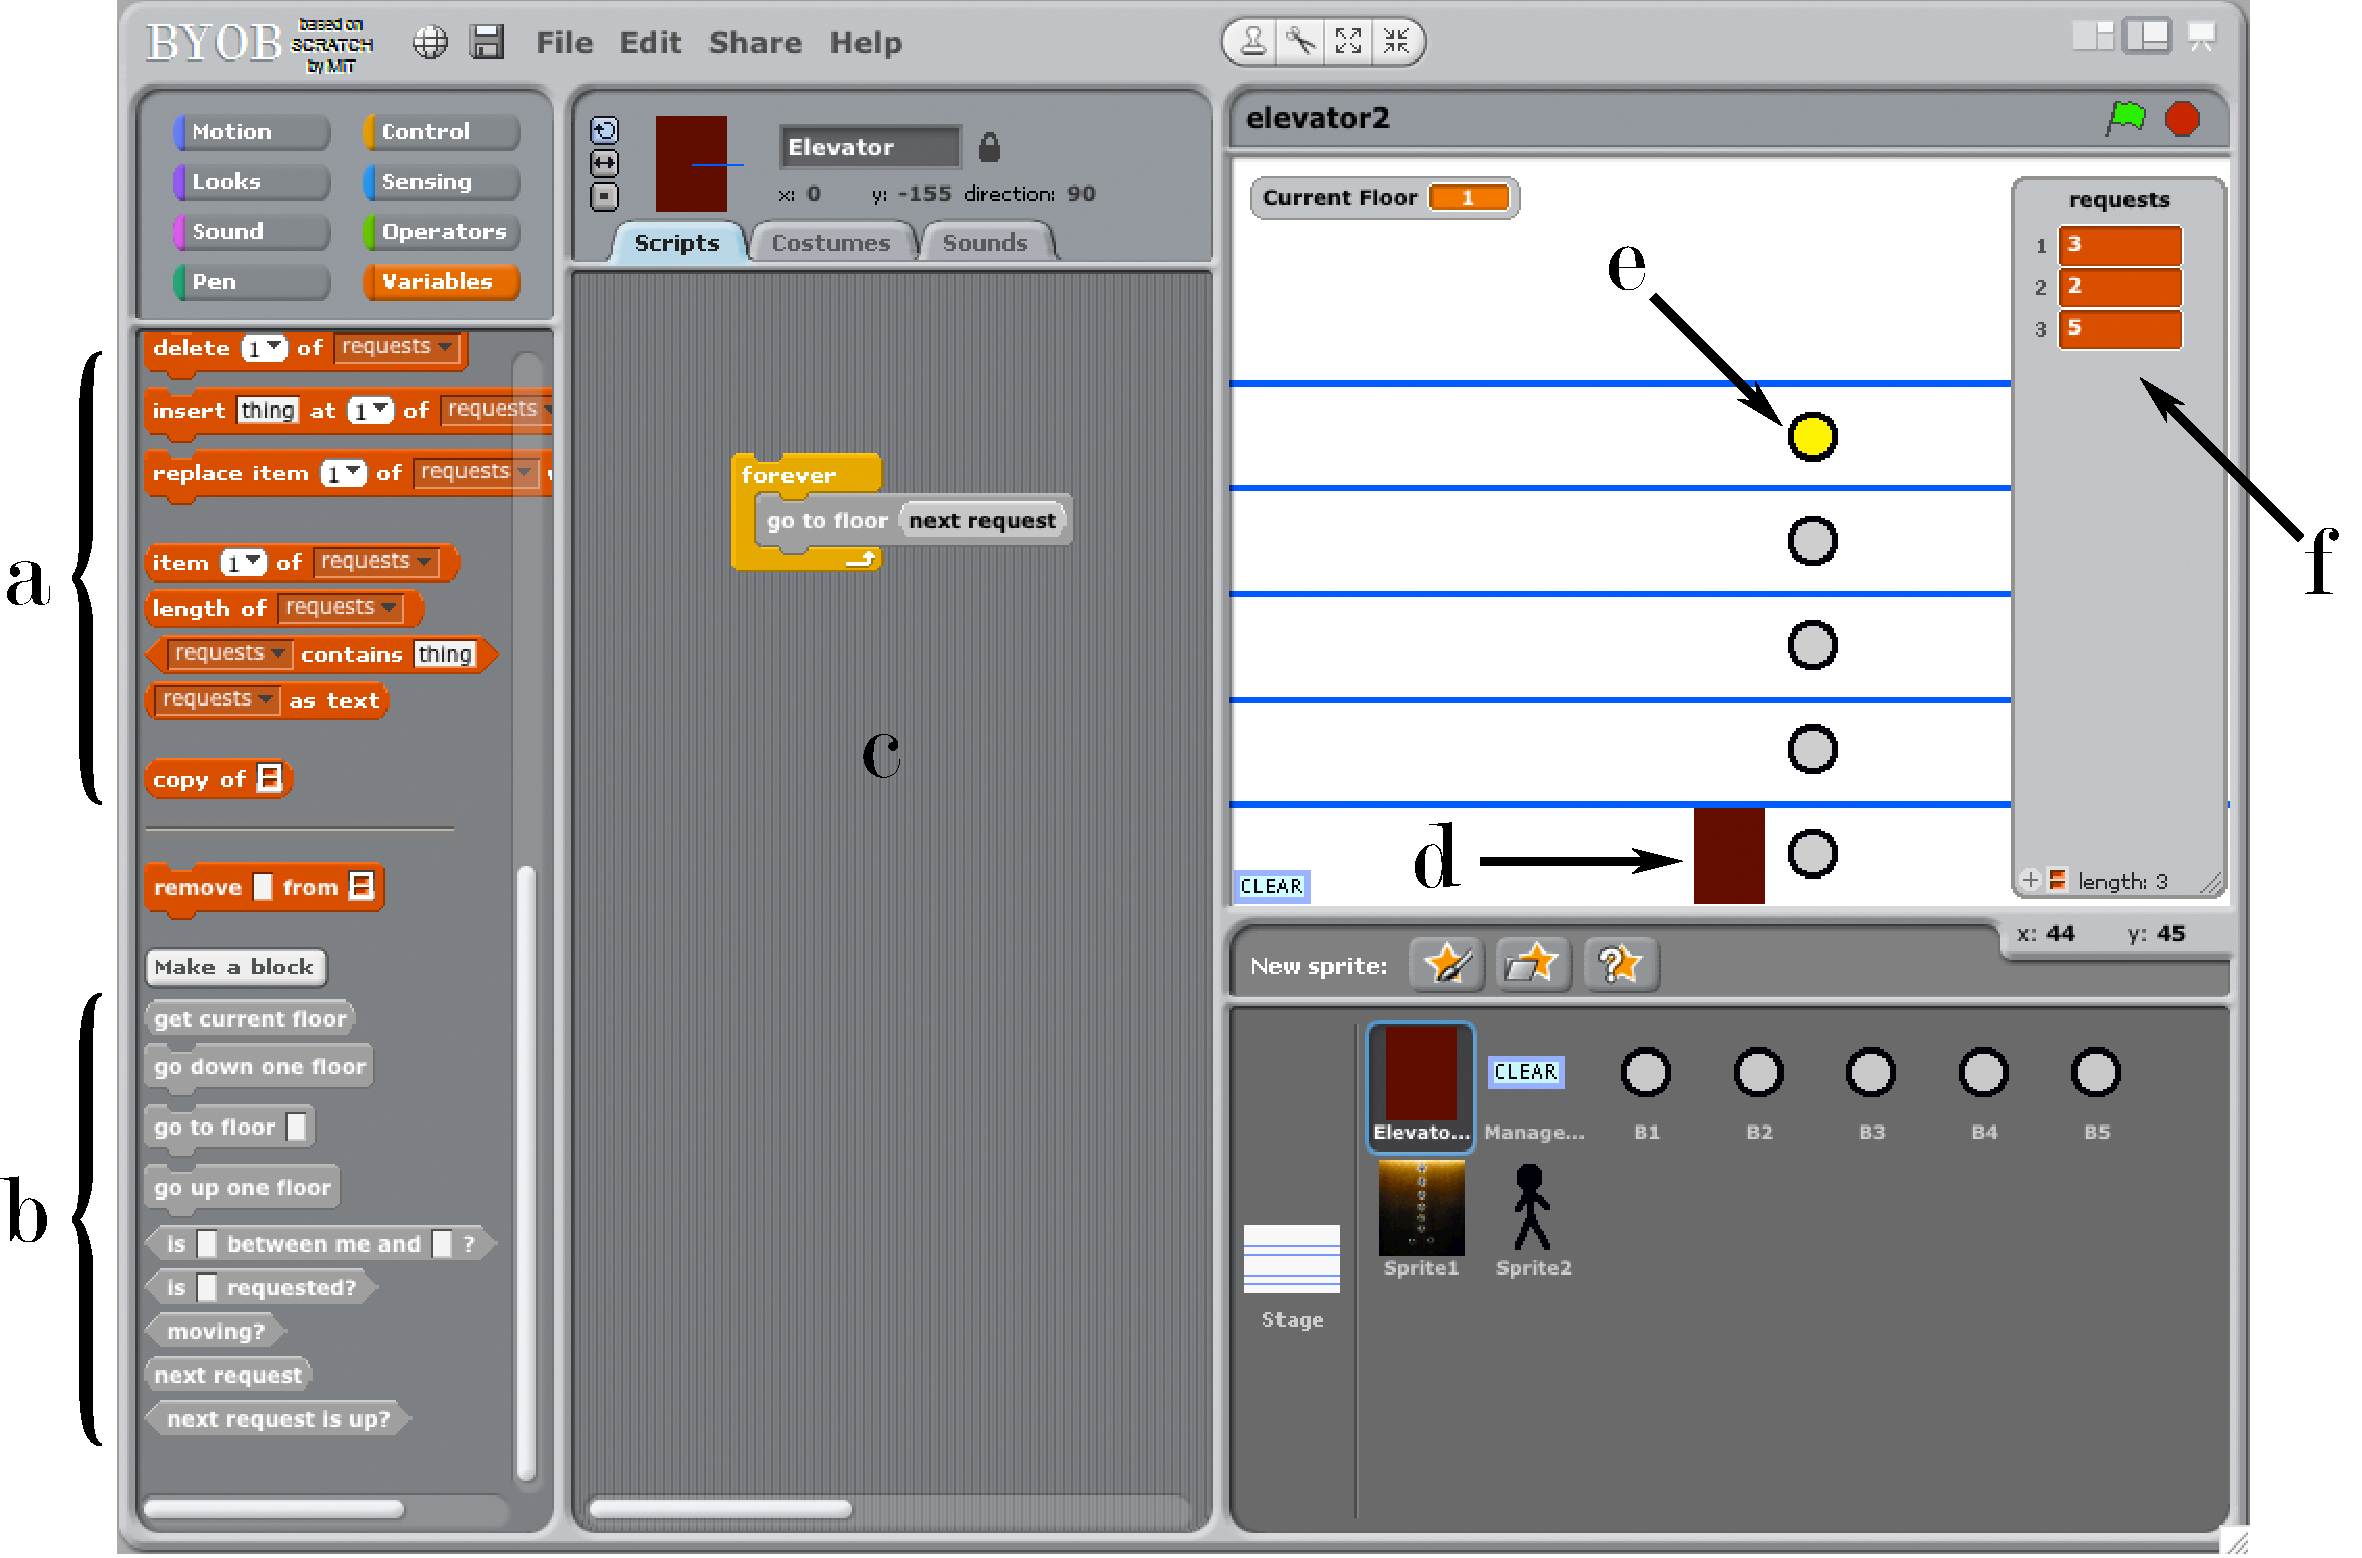
\includegraphics[width=\textwidth]{images/elevator/sim-labelled-3} %change to "-3bw" for bw
	\par\end{centering}
	\caption[Workspace for the Elevator Control microworld.]{
		Workspace for the Elevator Control microworld. The components of the environment are: (a) Standard programming primitives, including logic; (b) Custom procedures for elevator simulation; (c) Code workspace where the procedures are assembled into a program; (d) Graphical representation of the elevator; (e) Call buttons that add requests to the queue; (f) The request queue, showing three elements.
	}
	\label{fig:elevator-workspace}
	\end{figure}
	

	
	%
	\begin{figure}
	\begin{centering}
	\includegraphics{images/elevator_primitives}
	\par\end{centering}
	\caption[Custom procedures for elevator control.]{Custom procedures for elevator control that were built into the simulator.}
	\label{fig:elevator-blocks}
	\end{figure}
	
	\subsubsection{Purpose}
	
	This activity was intended to explore the students reactions to a difficult optimization problem. When the activity was conducted, students participated in ``problem-framing;" that is, making sense of the problem situation and forming their task goals. In this activity, the general goal was to create an improved elevator control program, but what needed to be ``improved" was not clear to the students until they conducted sufficient ``problem-framing." Unique among the other sessions, this activity encouraged students to think and work purely symbolically, where the tools and materials they manipulated were all abstract representations of real-world items.
	
	
	\subsubsection{Protocol}
	
	The students were given the goal of developing an algorithm to control an elevator. The concept of simulation was introduced, as was the Scratch programming language subset used by the simulator.
	
	The students were provided with a simple but working starter solution,
	shown in Figure~\ref{fig:elevator-trivial}. The first challenge for the students was to understand why the given solution worked and why it was sub-optimal.
	There was no formal mechanism to prevent students from working
	on a solution before they fully understand the problem, but they were prompted often by researchers to establish their current understanding
	of the situation.
	
	The provided solution called the elevator to travel to the next floor to which it was called, in the order that the calls were made. The major flaw of
	this solution was that people who were waiting for service were passed
	by the elevator as it traveled blindly to the called floor. This inefficiency would result in unacceptable wait times (and therefore unhappy people), as well as unnecessary energy expenditure
	by the building owner.
	
	%
	\begin{figure}
	\begin{centering}
	\includegraphics{images/elevator-trivial-solution}
	\par\end{centering}
	\caption[Starter solution of the Elevator Control problem.]{Starter solution of the Elevator Control problem. The ``forever'' structure will infinitely loop whatever code block sequence is nested within it. In this case, the only action is to ``go to floor'' with an argument of ``next request." The elevator will continually go to floor whose request is at the top of the queue.}
	\label{fig:elevator-trivial}
	\end{figure}
	
	\subsubsection{Rationale}
	
	This activity is abstract, and requires students to manipulate a system by means of symbolic representation. It also requires understanding of a queue structure,
	positional queries, and boolean logic. These latter elements are part of
	the everyday problems posed by both researching and practicing computer
	scientists and engineers. Control elements, such as determining location
	and direction of travel, are specifically common to robotics.




%%%%%%%%%%%%%%%%%%%%%%%%%%%%%%%%%%%%%%%%%%%Analysis
%%%%%%%%%%%%%%%%%%%%%%%%%%%%%%%%%%%%%%%%%%%Plan
\section{Coding and Analysis} \label{sec:analysis-plan}
Videos from student sessions were analyzed using coding techniques informed by \citet{welch} and \citet{REESE}, where specific codes were defined to describe important behaviors. Additional codes were created in the style of grounded theory \citep{strauss97}: as behaviors and patterns that were not predicted were observed. 

The body of codes covered a wide range of design behaviors, as seen in Appendix~\ref{tab:starting-codes}, but only the TEST code was used in analysis, as it was used to characterize design iteration. 

Analysis was done initially with all of the codes using NVIVO software. Codes were applied to specific time spans of the video where the corresponding behavior or activity was observed. A second phase of analysis was conducted that only included codes that represented testing. This phase generated greater detail and did not use NVIVO.

Data were analyzed to reveal trends in two directions. The first was to show trends across all students within each activity. The second was to show trends within each student across all activities.